%%%%%%%%%%%%%%%%%%%%%%%%%%%%%%%%%%%%%%%%%%%%%%%%%%%%%%%%%%%%%%%%%%%%%%
%%	Name: "Signal analysis template"
%%	File name: signalanalysis_template_main
%%	Version: 1.5
%%
%%	Compiler: XeLaTeX
%%
%%%%%%%%%%%%%%%%%%%%%%%%%%%%%%%%%%%%%%%%%%%%%%%%%%%%%%%%%%%%%%%%%%%%%%

\documentclass[conference,compsoc,onecolumn]{IEEEtran}

% *** LANGUAGE UTILITY PACKAGES ***
\usepackage[utf8]{inputenc} % Required for including letters with accents
\usepackage[spanish]{babel}

% *** USED PACKAGES ***
% *** MISC UTILITY PACKAGES ***
\usepackage{comment}			% Agregar comentarios
\usepackage{lipsum}				% Inserts dummy text
\usepackage{blindtext}
\usepackage{listings}					% Coding
\usepackage{verbatim}				% Verbatim
\usepackage[final]{pdfpages}
\usepackage{booktabs,dcolumn}
\usepackage{pdflscape}
\usepackage{afterpage}
%\setlist[itemize]{noitemsep, nolistsep}
\usepackage[bookmarks=false]{hyperref}
\usepackage{tcolorbox}									% Coloured boxes, for LATEX examples and theorems, etc
\usepackage{color}
\usepackage{xcolor} % Required for specifying colors by name									% Color packages foreground and back­ground color man­age­men
% *** CITATION PACKAGES ***
\usepackage{cite}
% *** GRAPHICS RELATED PACKAGES ***
\usepackage{graphicx}
\usepackage{caption}
\usepackage{pgfplots}
\usepackage{tikz}
\usetikzlibrary{shapes,arrows}
\usetikzlibrary{decorations.pathmorphing} % noisy shapes
\usetikzlibrary{fit}					% fitting shapes to coordinates
\usetikzlibrary{backgrounds}	% drawing the background after the foreground
\pgfplotsset{compat=1.13}
% *** MATH PACKAGES ***
\usepackage{amsmath}
\usepackage{mathtools}
\usepackage{amssymb}
\usepackage{amsfonts}
\usepackage{expl3}
\usepackage{bm}

% *** SPECIALIZED LIST PACKAGES ***
\usepackage{algorithmic}
\usepackage{listings}					% Coding
\usepackage[framed,numbered,autolinebreaks,useliterate]{mcode}
% *** ALIGNMENT PACKAGES ***
\usepackage{array}
% *** SUBFIGURE PACKAGES ***
%\ifCLASSOPTIONcompsoc
%\usepackage[caption=false,font=normalsize,labelfont=sf,textfont=sf]{subfig}
%\else
%\usepackage[caption=false,font=footnotesize]{subfig}
%\fi
% *** FLOAT PACKAGES ***
\usepackage{fixltx2e}
\usepackage{stfloats}
%\fnbelowfloat
%\usepackage{dblfloatfix}
% *** PDF, URL AND HYPERLINK PACKAGES ***
\usepackage{url}
\usepackage{everypage}


\usepackage{multirow} % In order to be able to insert rows spanning multiple lines
\usepackage{verbatim}
\usepackage[all]{xy}
\usepackage{listings}
\usepackage{subfigure}
\usepackage{multibib}
\usepackage{setspace} 
\usepackage{algorithm}			    	  % To insert nice algorithms

% *** CARPETA DONDE SE GUARDARAN LAS IMAGENES ***
\graphicspath{{figures/}}

% *** NUEVOS COMANDOS Y CONFIGURACIONES VARIAS ***
\interdisplaylinepenalty=2500
\newcommand{\Lpagenumber}{\ifdim\textwidth=\linewidth\else\bgroup
	\dimendef\margin=0
	\ifodd\value{page}\margin=\oddsidemargin
	\else\margin=\evensidemargin
	\fi
	\raisebox{\dimexpr -\topmargin-\headheight-\headsep-0.5\linewidth}[0pt][0pt]{%
		\rlap{\hspace{\dimexpr \margin+\textheight+\footskip}%
			\llap{\rotatebox{90}{\thepage}}}}%
	\egroup\fi}

\AddEverypageHook{\Lpagenumber}%

\newcommand{\newtxt}[1]{\textcolor{black}{#1}}
\renewcommand\IEEEkeywordsname{Palabras cláve:}
\newcommand{\mx}[1]{\mathbf{\bm{#1}}} % Matrix command
\newcommand{\vc}[1]{\mathbf{\bm{#1}}} % Vector command
\newcommand{\linebreakand}{%
  \end{@IEEEauthorhalign}
  \hfill\mbox{}\par
  \mbox{}\hfill\begin{@IEEEauthorhalign}
}

%% Separación de palabras
\hyphenation{op-tical net-works semi-conduc-tor HHMMSS}


\begin{document}

% *** TITLES AND NAMES ***
% title of the document
\title{Proyecto 1: Plataforma de seguimiento de datos COVID-19 para Colombia}
% author names and affiliations
\author{\IEEEauthorblockN{Laura Camila Blanco Gómez}
\IEEEauthorblockA{\textit{Escuela de Ciencias Exactas e Ingeniería}\\
	Universidad Sergio Arboleda - Bogotá, Colombia\\
	laura.blanco01@correo.usa.edu.co}
	\and
\IEEEauthorblockN{Santiago Cáceres Linares}
\IEEEauthorblockA{\textit{Escuela de Ciencias Exactas e Ingeniería}\\
	Universidad Sergio Arboleda - Bogotá, Colombia\\
	santiago.caceres01@correo.usa.edu.co}
	\linebreakand
	\IEEEauthorblockN{Andrés Camilo López Ramírez}
\IEEEauthorblockA{\textit{Escuela de Ciencias Exactas e Ingeniería}\\
	Universidad Sergio Arboleda - Bogotá, Colombia\\
	andres.lopez01@correo.usa.edu.co}
	}


% *** MAKE TITLE ***
\maketitle
\IEEEoverridecommandlockouts
\IEEEpeerreviewmaketitle

\begin{abstract}
En el presente proyecto se busca extraer diversos datos sobre el virus COVID-19 de una página web, guardarlos en una base de datos y representar de forma selectiva mediante gráficos de tortas, gráficos de dos dimensiones y diagramas de barras de los datos que se han extraidos de la página web.
\end{abstract}


\begin{IEEEkeywords}
    COVID19, Colombia, Web Scraping, Python, html.
\end{IEEEkeywords}


\section{Marco teórico}
\label{sec:introduction}
\subsection{COVID19} 
El COVID‑19 es la enfermedad infecciosa causada por el coronavirus que se ha descubierto más recientemente y afecta a muchos países de todo el mundo.Razon por la cual fue ´
clasificado como Pandemia por la Organizacion Mundial de la Salud (OMS).

La mayoría de las personas (alrededor del 80\%) se recuperan de la enfermedad sin necesidad de tratamiento hospitalario.  Alrededor de 1 de cada 5 personas que contraen la COVID‑19 acaba presentando un cuadro grave y experimenta dificultades para respirar.

Actualmente en Colombia se cuentan con 818.203 casos confirmados, de los cuales 68.308 son casos activos, 722.536 personas recuperadas y 25.641 fallecidos.
\hfill \break
\subsection{Web scraping} 
Es una técnica que permite extraer datos e información de una web. Este tutorial es una guía de inicio al web scraping con Python, utilizando para ello la librería Beautiful Soup.

Beautiful Soup es una librería Python que permite extraer información de contenido en formato HTML o XML.

Se deben seguir los siguentes pasos para un buen funcionamiento del web scraping:
\begin{itemize}
\item Identifica los elementos de la página de los que extraer la información
\item Descarga el contenido de la página
\item Crear la «sopa»
\item Busca los elementos en la «sopa» y obtén la información deseada
 \end{itemize}


\section{Resultados}
Para realizar la extracción de datos se usa la técnica \textbf{Web Scraping}, con la cual se extrajo información  desde \textbf{Wikipedia}, ya que cuenta con tablas que muestran los valores de contagios, muertes, supervivencia y casos activos del COVID-19, estos se actualizan constantemente.
Para esto se hizo uso de las librerías de \textbf{BeautifulSoup} y \textbf{requests}.
\hfill \break


\lstset{language=Python, breaklines=true, basicstyle=\footnotesize}
\lstset{numbers=left, numberstyle=\tiny, stepnumber=1, numbersep=-2pt}
\begin{lstlisting}[frame=single,caption={Código del web scraping },captionpos=b]
 from bs4 import BeautifulSoup
 import requests
 import pandas as pd
 import numpy as np
 import matplotlib.pyplot as plt

 url = 'https://es.wikipedia.org/wiki/Pandemia_de_enfermedad_por_coronavirus_de_2020_en_Colombia'
 ruta = "/Users/andre/DatosCovid.CSV"

 page_response = requests.get(url, timeout=5)
 page_content = BeautifulSoup(page_response.content, "html.parser")
 ciudadtxt = list()
 numerosArray = list()

 tablaCol = page_content.find(
    "table", attrs={"class": "wikitable sortable col1izq"})
ciudadRows = tablaCol.find_all("tr")

 for row in ciudadRows:
    numerostd = row.find_all("td")[1:]
    for i in numerostd:
        numerosArray.append(sinEspacios(i.text))
    ciudadLink = row.find_all("a")
    for i in ciudadLink:
        ciudadtxt.append(i.text)



\end{lstlisting}
\label{cod}

Después de hacer la extración de datos se hace una "divición" de esta información que se encuentra en \textbf{numerosArray}, esto se hizo por medio de varias listas como se ve en el siguiente código, para después guardar toda esta información de un \textbf{DataFrame}

\lstset{language=Python, breaklines=true, basicstyle=\footnotesize}
\lstset{numbers=left, numberstyle=\tiny, stepnumber=1, numbersep=-2pt}
\begin{lstlisting}[frame=single,caption={Código división de información y DataFrame },captionpos=b]

 for i in range(0, 330, 10):
    total.append(numerosArray[i])
 total.reverse()

 for i in range(1, 330, 10):
    cxMhad.append(numerosArray[i])
 cxMhad.reverse()

 for i in range(2, 330, 10):
    muertesT.append(numerosArray[i])
 muertesT.reverse()

 for i in range(3, 330, 10):
    porjeMT.append(numerosArray[i])
 porjeMT.reverse()

 for i in range(4, 330, 10):
    falleMhab.append(numerosArray[i])
 falleMhab.reverse()

 for i in range(5, 330, 10):
    recuT.append(numerosArray[i])
 recuT.reverse()

 for i in range(6, 330, 10):
    porjeRT.append(numerosArray[i])
 porjeRT.reverse()

 for i in range(7, 330, 10):
    CasActT.append(numerosArray[i])
 CasActT.reverse()

 for i in range(8, 330, 10):
    porjeACT.append(numerosArray[i])
 porjeACT.reverse()

 for i in range(9, 330, 10):
    AxMhab.append(numerosArray[i])
 AxMhab.reverse()


 df = pd.DataFrame({'Nombre': ciudadtxt, 'Casos Confirmados Totales': total,                        'Casos por millon de habitantes': cxMhad,
                   'Muertes Totales': muertesT, 'Porcentaje de muertes': porjeMT, 'Fallecido por millon de habitantes': falleMhab,
                   'Recuperados Totales': recuT, 'Porcentaje de recuperados': porjeRT, 'Casos Activos Totales': CasActT,
                   'Porecentaje Casos Activos': porjeACT, 'Casos Activos por millon de habitantes': AxMhab})

\end{lstlisting}
\label{cod}

\begin{figure}[H]
    \centering
    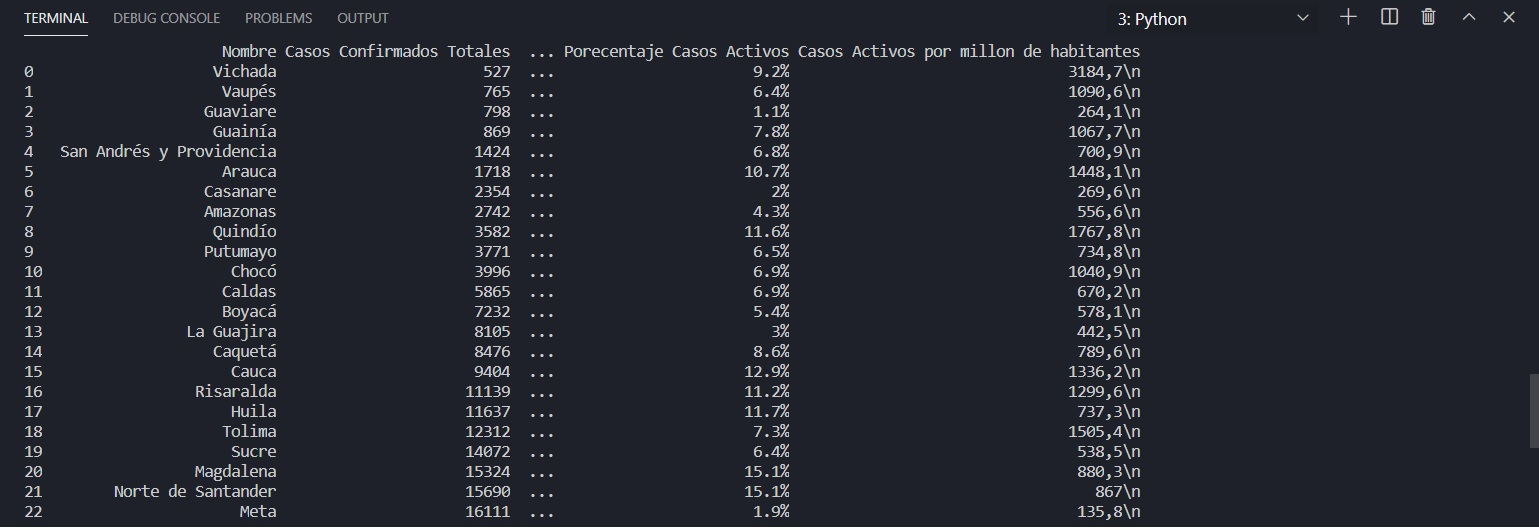
\includegraphics[keepaspectratio , scale = 0.3]{dataframe.jpg}
    \caption{DataFrame}\label{GraficoTorta}
\end{figure}

Para enviar los datos a la base de datos creamos una base de datos en MySQL, y desde Python se le enviaran los datos que debe crear en este caso en forma de tabla y definiendo el tipo de valor que se le envio y esta se llenara a partir de un for con los datos que se exportaron inicialmente desde la pagina web.


\lstset{language=Python, breaklines=true, basicstyle=\footnotesize}
\lstset{numbers=left, numberstyle=\tiny, stepnumber=1, numbersep=-2pt}
\begin{lstlisting}[frame=single,caption={Código base de datos },captionpos=b]
 #Nombre de las columnas
 Ciudad=flist[0][0]; Total_Casos_Confirmados=flist[0][1]; CasosxMillon=flist[0][2];  Total_Fallecimientos=flist[0][3]; Porcentaje_Fallecidos=flist[0][4];  FallecidosxMillon=flist[0][5]; Total_Recuperados=flist[0][6];  Porcentaje_Recuperados=flist[0][7]; Casos_Activos=flist[0][8];  Porecentaje_CasosActivos=flist[0][9]; Casos_ActivosxMillon=flist[0][10]

 queryCreateTable = """create table datoscovid(
                        {} varchar (50),
                        {} double,
                        {} double,
                        {} double,
                        {} varchar (50),
                        {} double,
                        {} double,
                        {} varchar (50),
                        {} double,
                        {} varchar (50),
                        {} double
                        )""".format(Ciudad, Total_Casos_Confirmados, CasosxMillon, Total_Fallecimientos, Porcentaje_Fallecidos, FallecidosxMillon, Total_Recuperados, Porcentaje_Recuperados, Casos_Activos, Porecentaje_CasosActivos, Casos_ActivosxMillon)

 cursor.execute(queryCreateTable)
 del flist [0]
 rows = ''
 for i in range(len(flist)-1):
    rows += "('{}', '{}', '{}', '{}','{}', '{}', '{}','{}','{}','{}','{}')".format(flist[i][0],flist[i][1],flist[i][2],flist[i][3],
                                      flist[i][4],flist[i][5],flist[i][6],flist[i][7],
                                      flist[i][8],flist[i][9],flist[i][10],)
    if i != len(flist) - 2:
        rows +=','
 dataInsert = "insert into datoscovid values" + rows

 try:
    cursor.execute(dataInsert)
    db.commit()
    print("Inserción de datos exitosa!")
 except:
    print("Error en conexión :c")
    db.rollback()

 db.close()
\end{lstlisting}
\label{cod}


\begin{figure}[H]
    \centering
    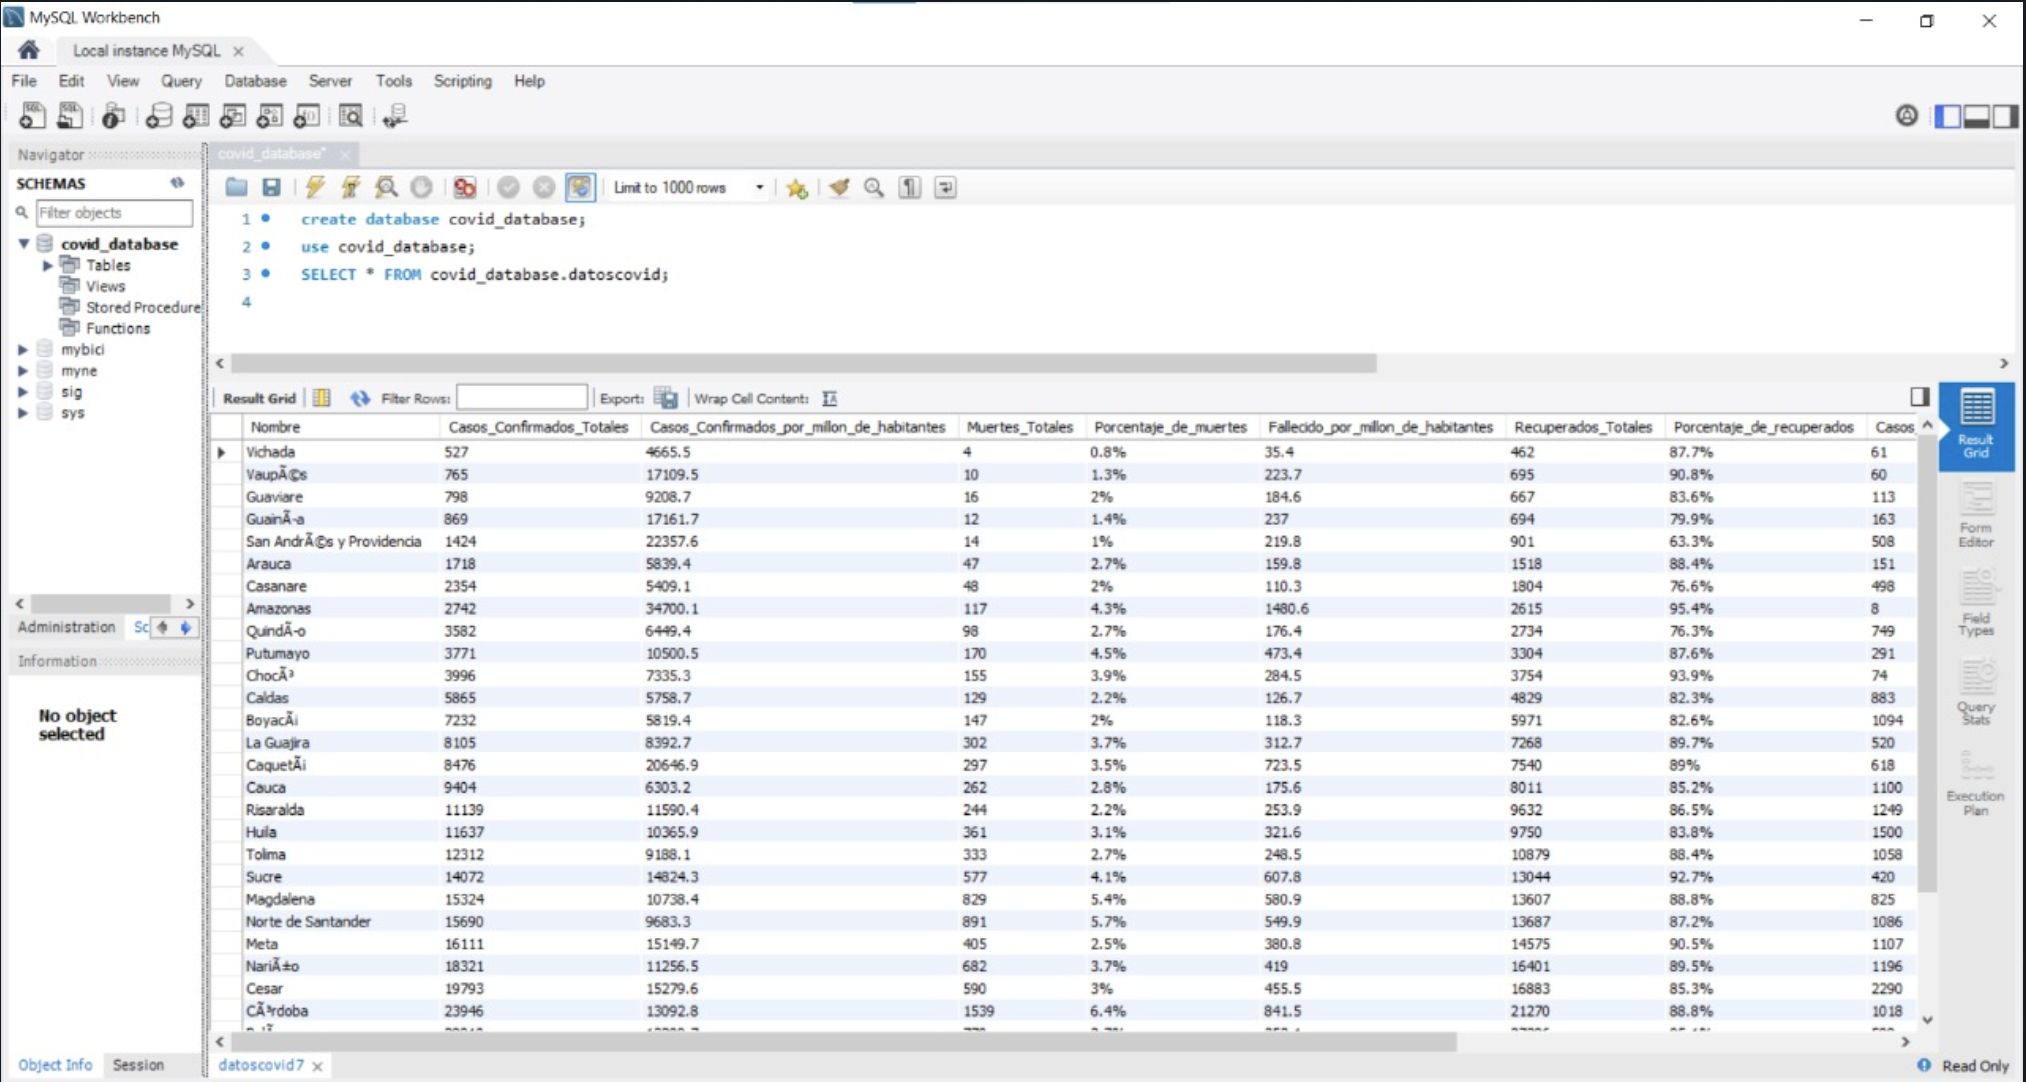
\includegraphics[keepaspectratio , scale = 0.5]{BaseDeDatos.png}
    \caption{Base de datos}\label{BaseDeDatos}
\end{figure}
Para representar la información extraída en graficas usamos el DataFrame para seleccionar los datos que queremos graficar y se guardan en  variables \textit{x}. y \textit{y}. Además se hace uso de la librería \textbf{matplotlib} para definir el tipo de grafica, en este caso es \textit{plt.pie()}.
\lstset{language=Python, breaklines=true, basicstyle=\footnotesize}
\lstset{numbers=left, numberstyle=\tiny, stepnumber=1, numbersep=-2pt}
\begin{lstlisting}[frame=single,caption={Código gráfica de barras },captionpos=b]
 # Grafica Barras
 x = df['Nombre'].iloc[28:33]
 y = df['Casos Confirmados Totales'].iloc[28:33]
 plt.bar(x, y)
 plt.xlabel('Departamenro')
 plt.ylabel('Casos Confirmados Totales')
 plt.grid()
 plt.show()
\end{lstlisting}
\label{cod}

\begin{figure}[H]
    \centering
    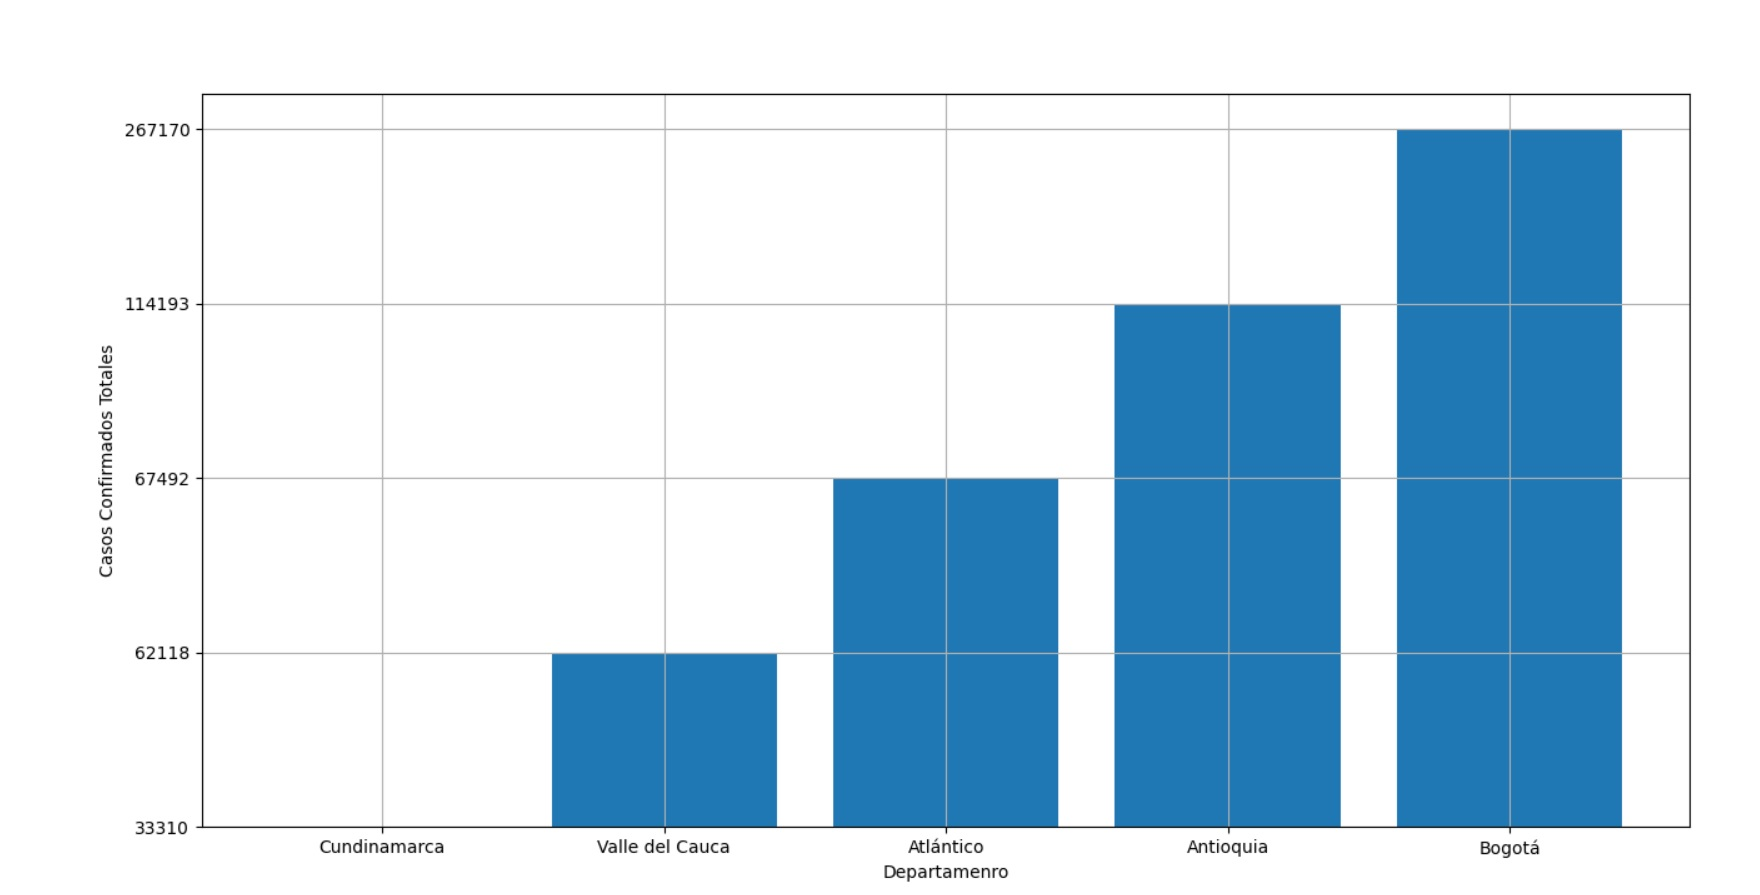
\includegraphics[keepaspectratio , scale = 0.3]{Grafica1.jpg}
    \caption{Grafico de barras}\label{GraficoBarras}
\end{figure}


En el caso de la gráfica de torta se hace uso del \textbf{plt.pie()} en el cual se encontrara \textit{autopct = "\%0.1f\%\%"}  el cual servirá para convertir los valores en porcentajes, aclarando que realizara esta conversián únicamente con los datos que se grafiquen.
\lstset{language=Python, breaklines=true, basicstyle=\footnotesize}
\lstset{numbers=left, numberstyle=\tiny, stepnumber=1, numbersep=-2pt}
\begin{lstlisting}[frame=single,caption={Código gráfica de torta },captionpos=b]
 #Grafico Torta 
 x = df['Muertes Totales'].iloc[28:33]
 y = df['Nombre'].iloc[28:33]
 plt.title('Muertes Totales')
 plt.pie(x,labels= y, autopct = "%0.1f%%"  )
 plt.show()
\end{lstlisting}
\label{cod}

\begin{figure}[H]
    \centering
    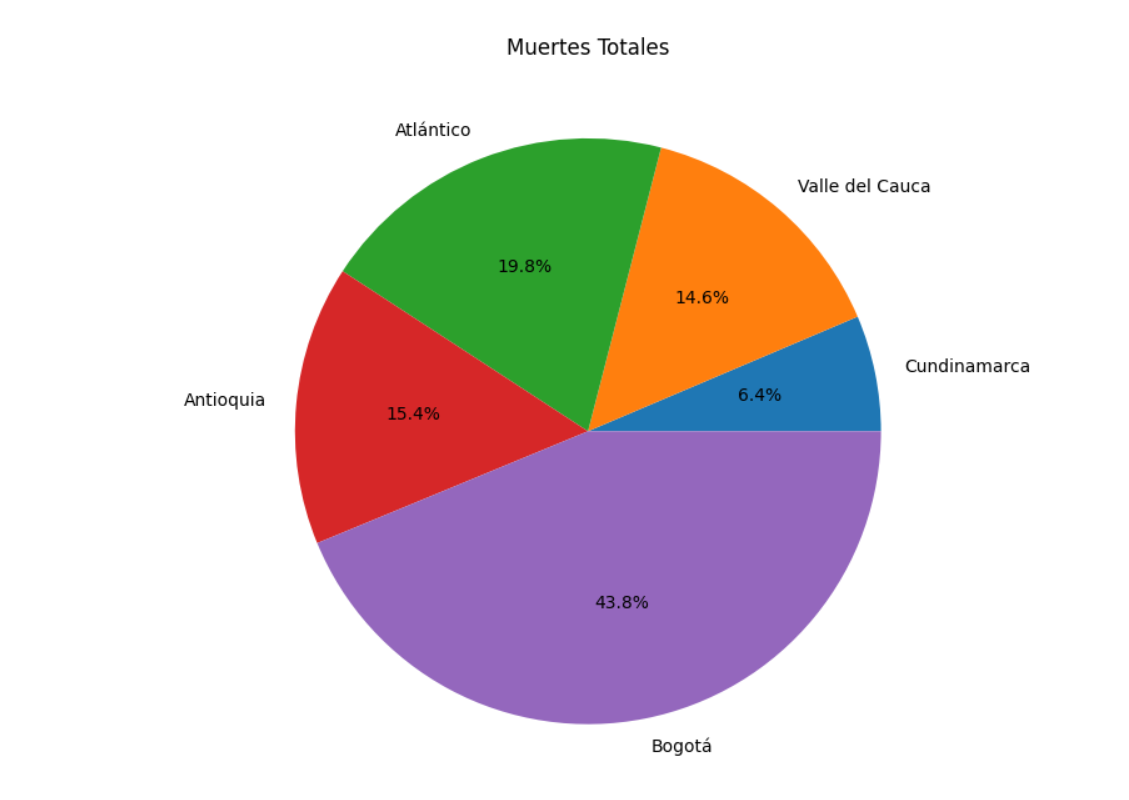
\includegraphics[keepaspectratio , scale = 0.3]{Grafica2.jpg}
    \caption{Grafico de torta}\label{GraficoTorta}
\end{figure}
Y por ultimo en el grafico 2D se usa \textbf{plt.plot()} y en nuestro caso hacemos uso de \textbf{plt.grid} para que se puedan apreciar las intersecciones de los valores en la recta.
\lstset{language=Python, breaklines=true, basicstyle=\footnotesize}
\lstset{numbers=left, numberstyle=\tiny, stepnumber=1, numbersep=-2pt}
\begin{lstlisting}[frame=single,caption={Código gráfica 2D },captionpos=b]
 #Grafico 2D
 x = df['Muertes Totales'].iloc[28:33]
 y = df['Nombre'].iloc[28:33]
 plt.plot(x,y)
 plt.xlabel('Casos Confirmados Totales')
 plt.ylabel('Departamenro')
 plt.grid()
 plt.show()
\end{lstlisting}
\label{cod}

\begin{figure}[H]
    \centering
    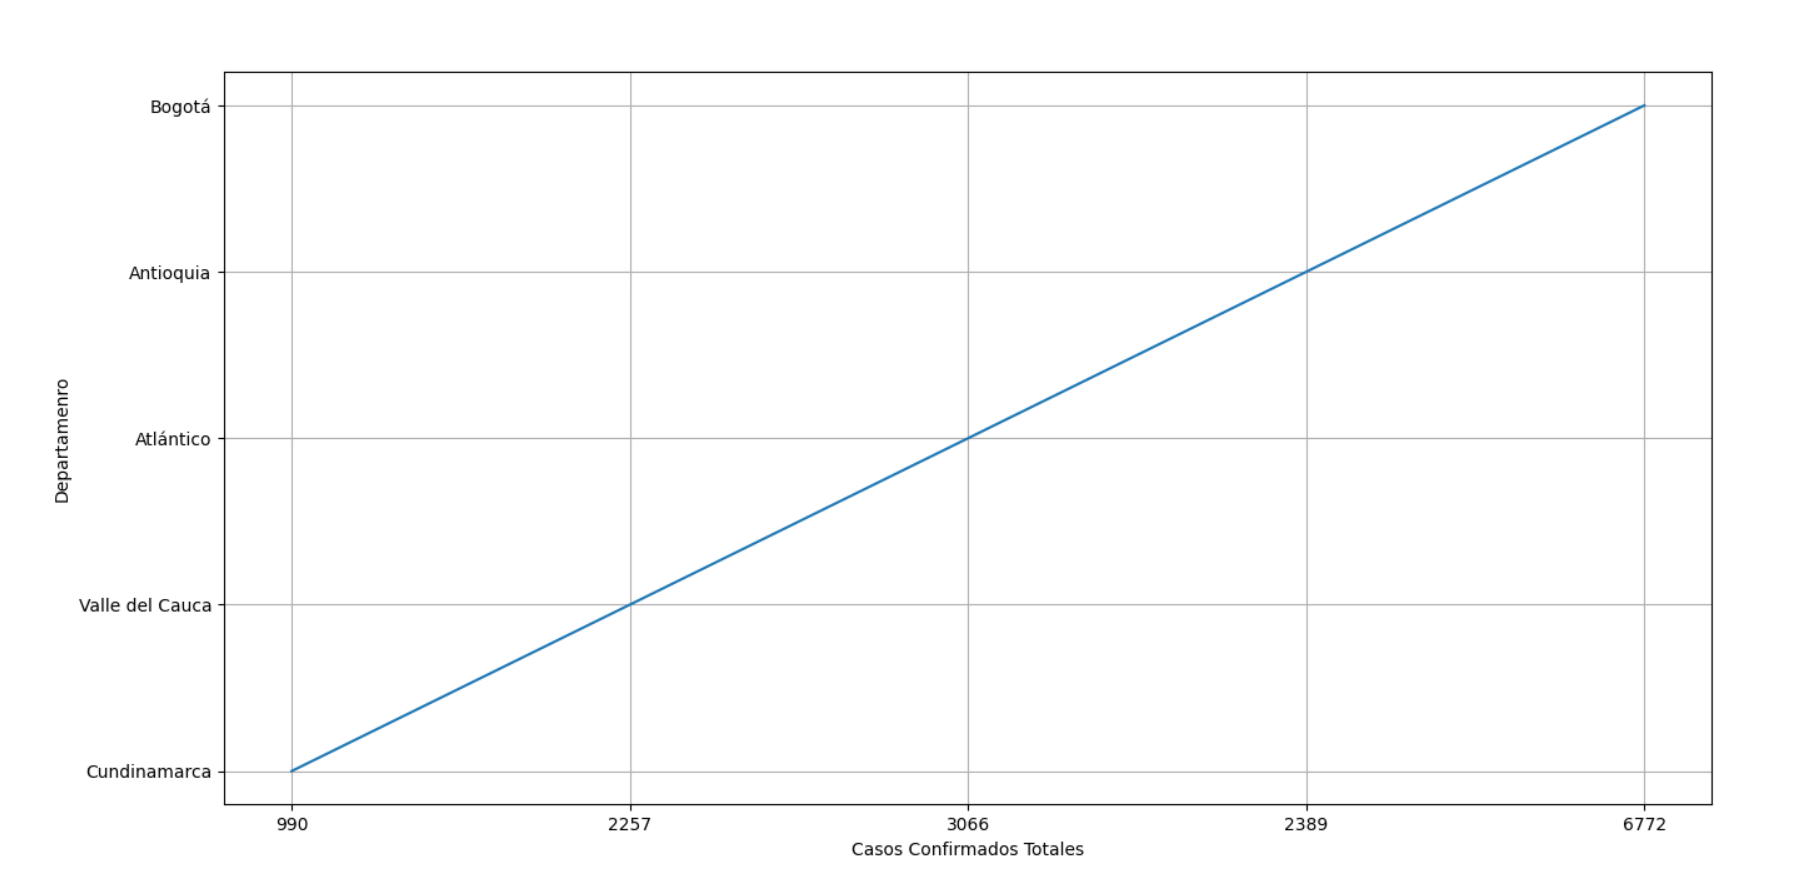
\includegraphics[keepaspectratio , scale = 0.3]{Grafica3.jpg}
    \caption{Grafico 2D}\label{Grafico2D}
    \label{sec:results}
\end{figure}

\section{Conclusiones}
\label{sec:conclusions}
\begin{itemize}
\item Conociendo la técnica de web scraping se facilito para la extracción desde la página web a Python.
\item Se utilizan las librerías de Python Pandas, beautifulsoap y request, ya que nos permiten crear DataFrames y archivos CSV, buscar información y buscar información del html respectivamente.
\item Se hace necesario a la hora de extraer los datos buscar páginas confiables que mantengan sus datos actualizados, ya que con estre se tendra un panorama más realista de lo que esta pasando.
\item Gracias al uso de los \textbf{DataFrame} se pudo almacenar de una manera facíl la información extraida para despues poder llevarla a un archivo CSV con el cual se lleno la base de datos posteriormente 

 \end{itemize}


\section{Link repositorio}
\label{sec:LinkRepositorio}
\url{https://github.com/ACLXRD/SA2020_G02_CovidScraper_6I3I11}


\nocite{*}
\bibliographystyle{IEEEtran}
\label{sec:biblio}
% Descomente y modiffique el archivo biblio.bib para agregar bibliografía
\bibliography{bib/biblio} 





%\pagestyle{empty}
\end{document}


